\input{header_xe.tex}
\def \labnum {2}
\def \labsubj {Теория автоматов}
\def \labauthor {Чебыкин И. Б.}
\def \labgroup {P3301}
\def \labinsp {Ожиганов А. А.}
\def \labname {Минимизация абстрактных автоматов \\ Вариант: 5}
\isnametrue

\usepackage{listings,longtable,amsmath,amsfonts,graphicx,tikz,tabularx,pgf,multirow}
\usepackage{caption}
\usetikzlibrary{arrows,automata}

\captionsetup{labelsep=period}
\pagestyle{fancy}
\begin{document}
\input{title.tex}

\section{Описание работы}
Цель -- овладение навыками минимизации полностью определенных абстрактных автоматов.
Абстрактный автомат задан табличным способом. Причем абстрактный автомат Мили
представлен таблицами переходов и выходов, а абстрактный автомат Мура -- одной
отмеченной таблицей переходов. Эквивалентные автоматы могут иметь различное
число состояний. В связи с этим возникает задача нахождения минимального
(с минимальным числом состояний) автомата в классе эквивалентных между собой
автоматов.

Для минимизации абстрактного автомата использовать алгоритм,
предложенный Ауфенкампом и Хоном. Основная идея алгоритма состоит в разбиении
всех состояний исходного абстрактного автомата на попарно не пересекаемые классы
эквивалентных состояний. После разбиения происходит замена каждого класса
эквивалентности одним состоянием. Получившийся в результате минимальный
абстрактный автомат имеет столько же состояний, на сколько классов
эквивалентности разбиваются состояния исходного абстрактного автомата.
\section{Порядок выполнения задания}
\begin{enumerate}
\item В соответствии с номером варианта выбрать
абстрактный автомат $S=(A,Z,W,\delta,\lambda,a_1)$.
\item Найти последовательные разбиения $\pi_1, \pi_2,..., \pi_k, \pi_k+1$
множества А на классы одно-, двух-, ... , $k+1$ -- эквивалентных между собой состояний.
\item Разбиение на классы производить до тех пор, пока на каком-то $k+1$ шаге
не окажется, что $\pi_k+1 = \pi_k.$
\item В каждом классе эквивалентности разбиения π выбрать по одному элементу,
которые образуют множество А' состояний минимального
автомата $S'=(A',Z,W,\delta',\lambda',a_1')$, эквивалентного исходному автомату S.
\item Функции переходов и выходов автомата S', определить на множестве A' *Z,
то есть $\delta'$ : A' *Z → A', $\lambda'$ : A' *Z → W.
\item В качестве $a_1'$, выбрать одно из состояний, эквивалентных $a_1$
\item Используя навыки полученные при выполнении практического задания 1,
осуществить проверку исходного и минимизированного автоматов на эквивалентность.
\end{enumerate}
\section{Выполнение}
\subsection{Исходный автомат}
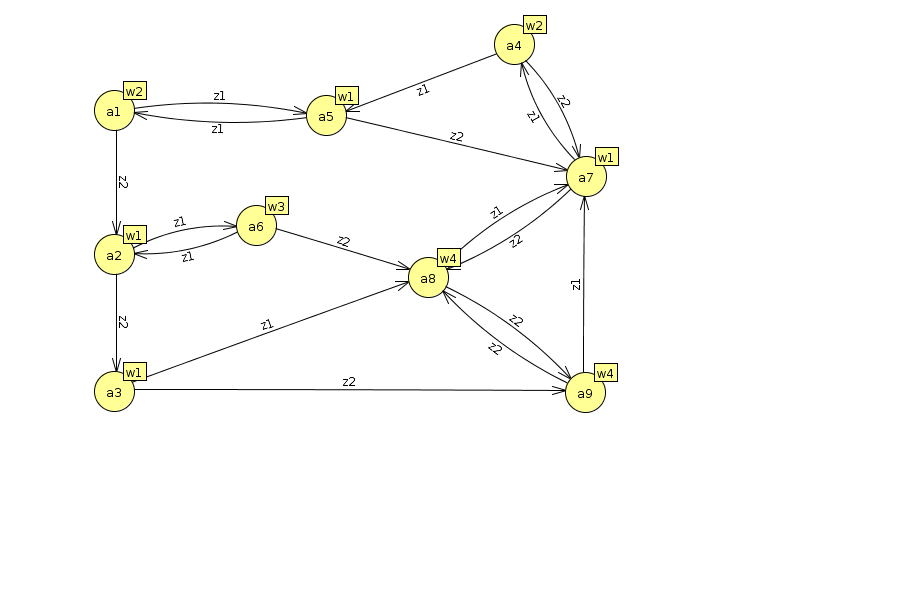
\includegraphics[width=400bp]{img/first.png}

\begin{table}[!h]
\begin{tabular}{|c|c|c|c|c|c|c|c|c|c|c|}
\hline
$\lambda$ & $w_2$ & $w_1$ & $w_1$ & $w_2$ & $w_1$ & $w_3$ & $w_1$ & $w_4$ & $w_4$ \\ \hline
$\delta$  & $a_1$ & $a_2$ & $a_3$ & $a_4$ & $a_5$ & $a_6$ & $a_7$ & $a_8$ & $a_9$ \\ \hline
$z_1$     & $a_5$ & $a_6$ & $a_8$ & $a_5$ & $a_1$ & $a_2$ & $a_4$ & $a_7$ & $a_7$ \\ \hline
$z_2$     & $a_2$ & $a_3$ & $a_9$ & $a_7$ & $a_7$ & $a_8$ & $a_8$ & $a_9$ & $a_8$ \\ \hline
\end{tabular}
\end{table}
\subsection{Минимизация}

$\pi_0 = A_1 \{a_1, a_4\}, B_1 \{a_2, a_3, a_5, a_7\}, C_1 \{a_6\}, E_1 \{a_8, a_9\}$

\begin{table}[!h]
\begin{tabular}{|c|c|c|c|c|c|c|c|c|c|c|}
\hline
$\pi$     & $a_1$ & $a_4$ & $a_2$ & $a_3$ & $a_5$ & $a_7$ & $a_6$ & $a_8$ & $a_9$ \\ \hline
$z_1$     & $B_1$ & $B_1$ & $C_1$ & $E_1$ & $A_1$ & $A_1$ & $B_1$ & $B_1$ & $B_1$ \\ \hline
$z_2$     & $B_1$ & $B_1$ & $B_1$ & $E_1$ & $B_1$ & $E_1$ & $E_1$ & $E_1$ & $E_1$ \\ \hline
\end{tabular}
\end{table}

$\pi_1 = A_2 \{a_1, a_4\}, B_2 \{a_2\}, C_2 \{a_3\}, D_2 \{a_5\}, E_2 \{a_7\}, F_2 \{a_6\}, G_2 \{a_8, a_9\}$

\begin{table}[!h]
\begin{tabular}{|c|c|c|c|c|c|c|c|c|c|c|}
\hline
$\pi$     & $a_1$ & $a_4$ & $a_2$ & $a_3$ & $a_5$ & $a_7$ & $a_6$ & $a_8$ & $a_9$ \\ \hline
$z_1$     & $D_2$ & $D_2$ & $F_2$ & $G_2$ & $A_2$ & $A_2$ & $B_2$ & $E_2$ & $E_2$ \\ \hline
$z_2$     & $B_2$ & $E_2$ & $C_2$ & $G_2$ & $E_2$ & $G_2$ & $G_2$ & $G_2$ & $G_2$ \\ \hline
\end{tabular}
\end{table}

$\pi_2 = A_3 \{a_1\}, B_3 \{a_2\}, C_3 \{a_3\}, D_3 \{a_5\}, E_3 \{a_7\}, F_3 \{a_6\}, G_3 \{a_8, a_9\}, H_3 \{a_4\}$

\begin{table}[!h]
\begin{tabular}{|c|c|c|c|c|c|c|c|c|c|c|}
\hline
$\pi$     & $a_1$ & $a_2$ & $a_3$ & $a_5$ & $a_7$ & $a_6$ & $a_8$ & $a_9$ & $a_4$ \\ \hline
$z_1$     & $D_3$ & $F_3$ & $G_3$ & $A_3$ & $H_3$ & $B_3$ & $E_3$ & $E_3$ & $D_3$ \\ \hline
$z_2$     & $B_3$ & $C_3$ & $G_3$ & $E_3$ & $G_3$ & $G_3$ & $G_3$ & $G_3$ & $E_3$ \\ \hline
\end{tabular}
\end{table}

$\pi_3 = A_4 \{a_1\}, B_4 \{a_2\}, C_4 \{a_3\}, D_4 \{a_5\}, E_4 \{a_7\}, F_4 \{a_6\}, G_4 \{a_8, a_9\}, H_4 \{a_4\}$

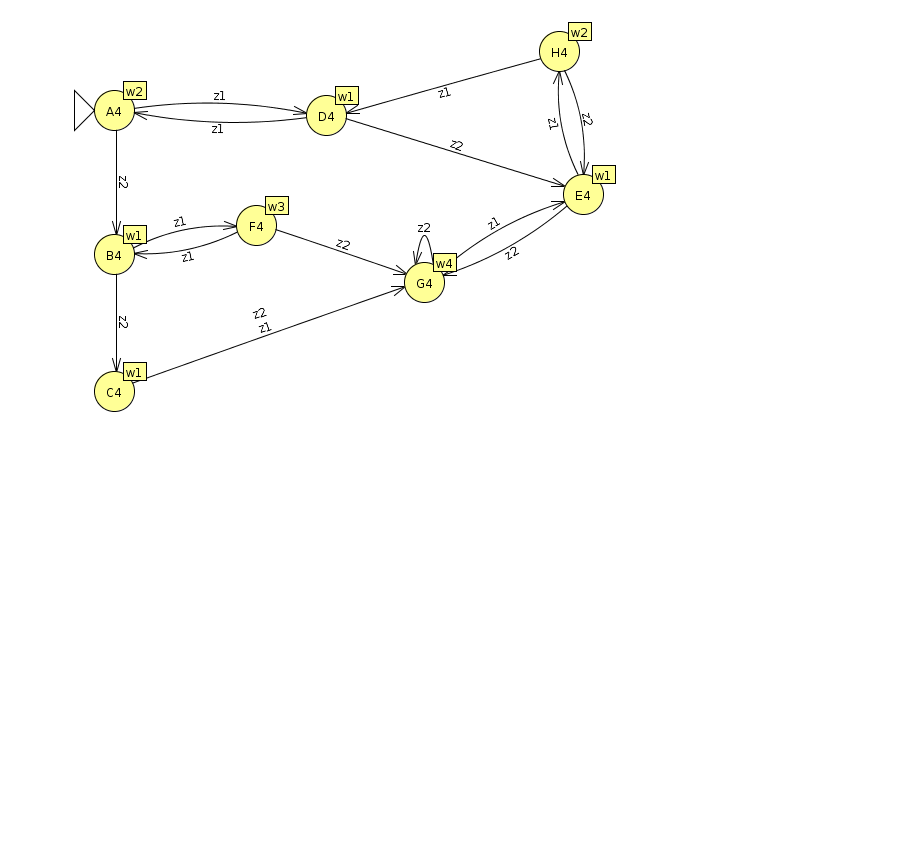
\includegraphics[width=400bp]{img/second.png}

\section{Проверка на эквивалентность}
\begin{table}[!h]
\tiny
\resizebox{\textwidth}{!}{\begin{tabular}{|c|c|c|c|c|c|c|c|c|c|c|c|c|c|c|c|c|c|c|c|c|}
\hline
\multicolumn{2}{|c|}{Входящий сигнал}        &    & z1 & z2 & z1 & z2 & z1 & z1 & z1 & z2 & z1 & z1 & z2 & z1 & z1 & z2 & z2 & z2 & z2 & z1 \\ \hline
\multirow{2}{*}{Состояние}            & Исх. & a1 & a5 & a7 & a4 & a7 & a4 & a5 & a1 & a2 & a6 & a2 & a3 & a8 & a7 & a8 & a9 & a8 & a9 & a7 \\ \cline{2-21}
                                      & Мин. & A4 & D4 & E4 & H4 & E4 & H4 & D4 & A4 & B4 & F4 & B4 & C4 & G4 & E4 & G4 & G4 & G4 & G4 & E4 \\ \hline

\multirow{2}{*}{Выходящий сигнал}     & Исх. & w2 & w1 & w1 & w2 & w1 & w2 & w1 & w2 & w1 & w3 & w1 & w1 & w4 & w1 & w4 & w4 & w4 & w4 & w1 \\ \cline{2-21}
                                      & Мин. & w2 & w1 & w1 & w2 & w1 & w2 & w1 & w2 & w1 & w3 & w1 & w1 & w4 & w1 & w4 & w4 & w4 & w4 & w1 \\ \hline
\end{tabular}}
\end{table}
\section{Вывод}
В ходе данной лабораторной работы была произведена минимизация автомата Мура.
Также было доказано, что исходный и получившийся автомат эквивалентны друг другу.
\end{document}
